\section{Code validation}
Every time a physicist implements a model, it is important to verify that the implementation is correct. New models that describe unknown areas of physics (such as new length scales) might be difficult to confirm if there are no experiments or comparable models available. 
\subsection{Maxwell-Boltzmann velocity distribution}

\subsection{Poiseuille velocity profile}
\label{sec:dsmc_validation_poiseuille}
The Poiseuille flow through a long channel is a standard and fundamental problem that is wideley studied in the gas dynamics literature. The system consists of two infinite parallel plates, displaced by a distance $h$. A pressure gradient is applied in the $z$-direction by a constant acceleration $g$, see figure \ref{fig:dsmc_validation_poiseuille_system}. 

\begin{figure}[htp]
\centering
%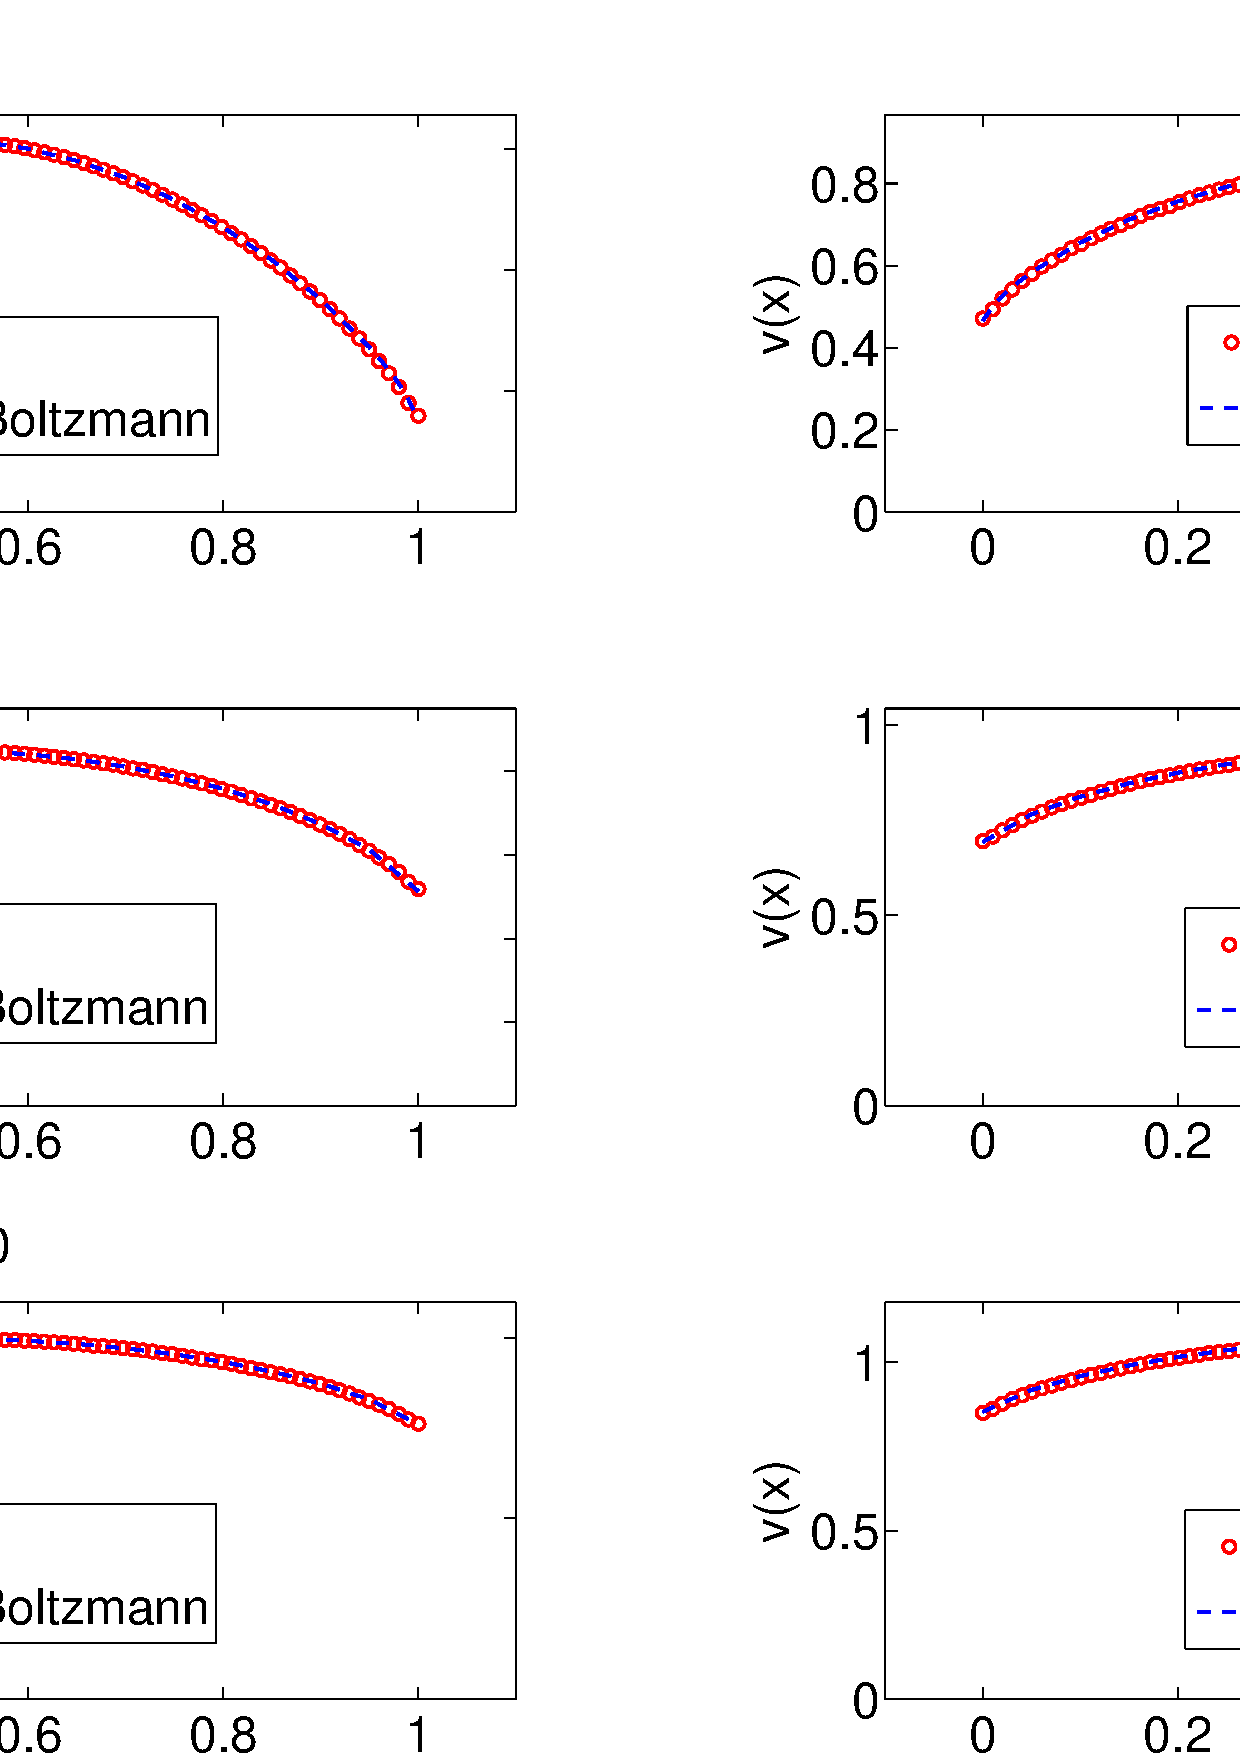
\includegraphics[scale=0.25]{figures/validation_poiseuille.pdf}
\label{fig:dsmc_validation_poiseuille_system}
\caption{Acceleration driven Poiseuille flow}
\end{figure}
The channel is periodic in the $x-$ and $z-$direction, emulating a large system with negligible boundary effects. The gas molecules collide with the plates through the thermal wall model, so the reflected particles will have zero tangential velocity on average. In the continuum limit, $Kn\rightarrow 0$, we expect the velocity profile to approach the parabolic solution \cite{batchelor2000introduction}
\begin{align}
	v_z(y) = \nabla P\frac{1}{2\mu}y(y-h).
\end{align}
However, in the transition flow regime, $0.1 \leq Kn \leq 10$, we expect a non zero slip velocity\cite{morris1992slip}. The Knudsen number will affect the velocity distribution through the fact that a high Knudsen number means a larger mean free path, hence fewer inter-molecular collisions. A low collision rate will make the surface effects propagate slower through the system. Ohwada et al. \cite{ohwada1989numerical} studied the Poiseuille flow for hard-sphere molecules with a wide range of Knudsen numbers by numerically solving the linearized Boltzmann equation. By using nondimensionalized units, the result is not dependent on the pressure difference or the temperature. The only assumption is that the pressure gradient is so small that the Boltzmann equation can be linearized around the equilibrium state. To setup as system like this is a simple task with the DSMC algorithm, and is a good test case to validate the code. In figure \ref{fig:dsmc_validation_poiseuille} we see that the DSMC model is in excellent agreement with the solutions obtained by Ohwada et al.
\begin{figure}[h]
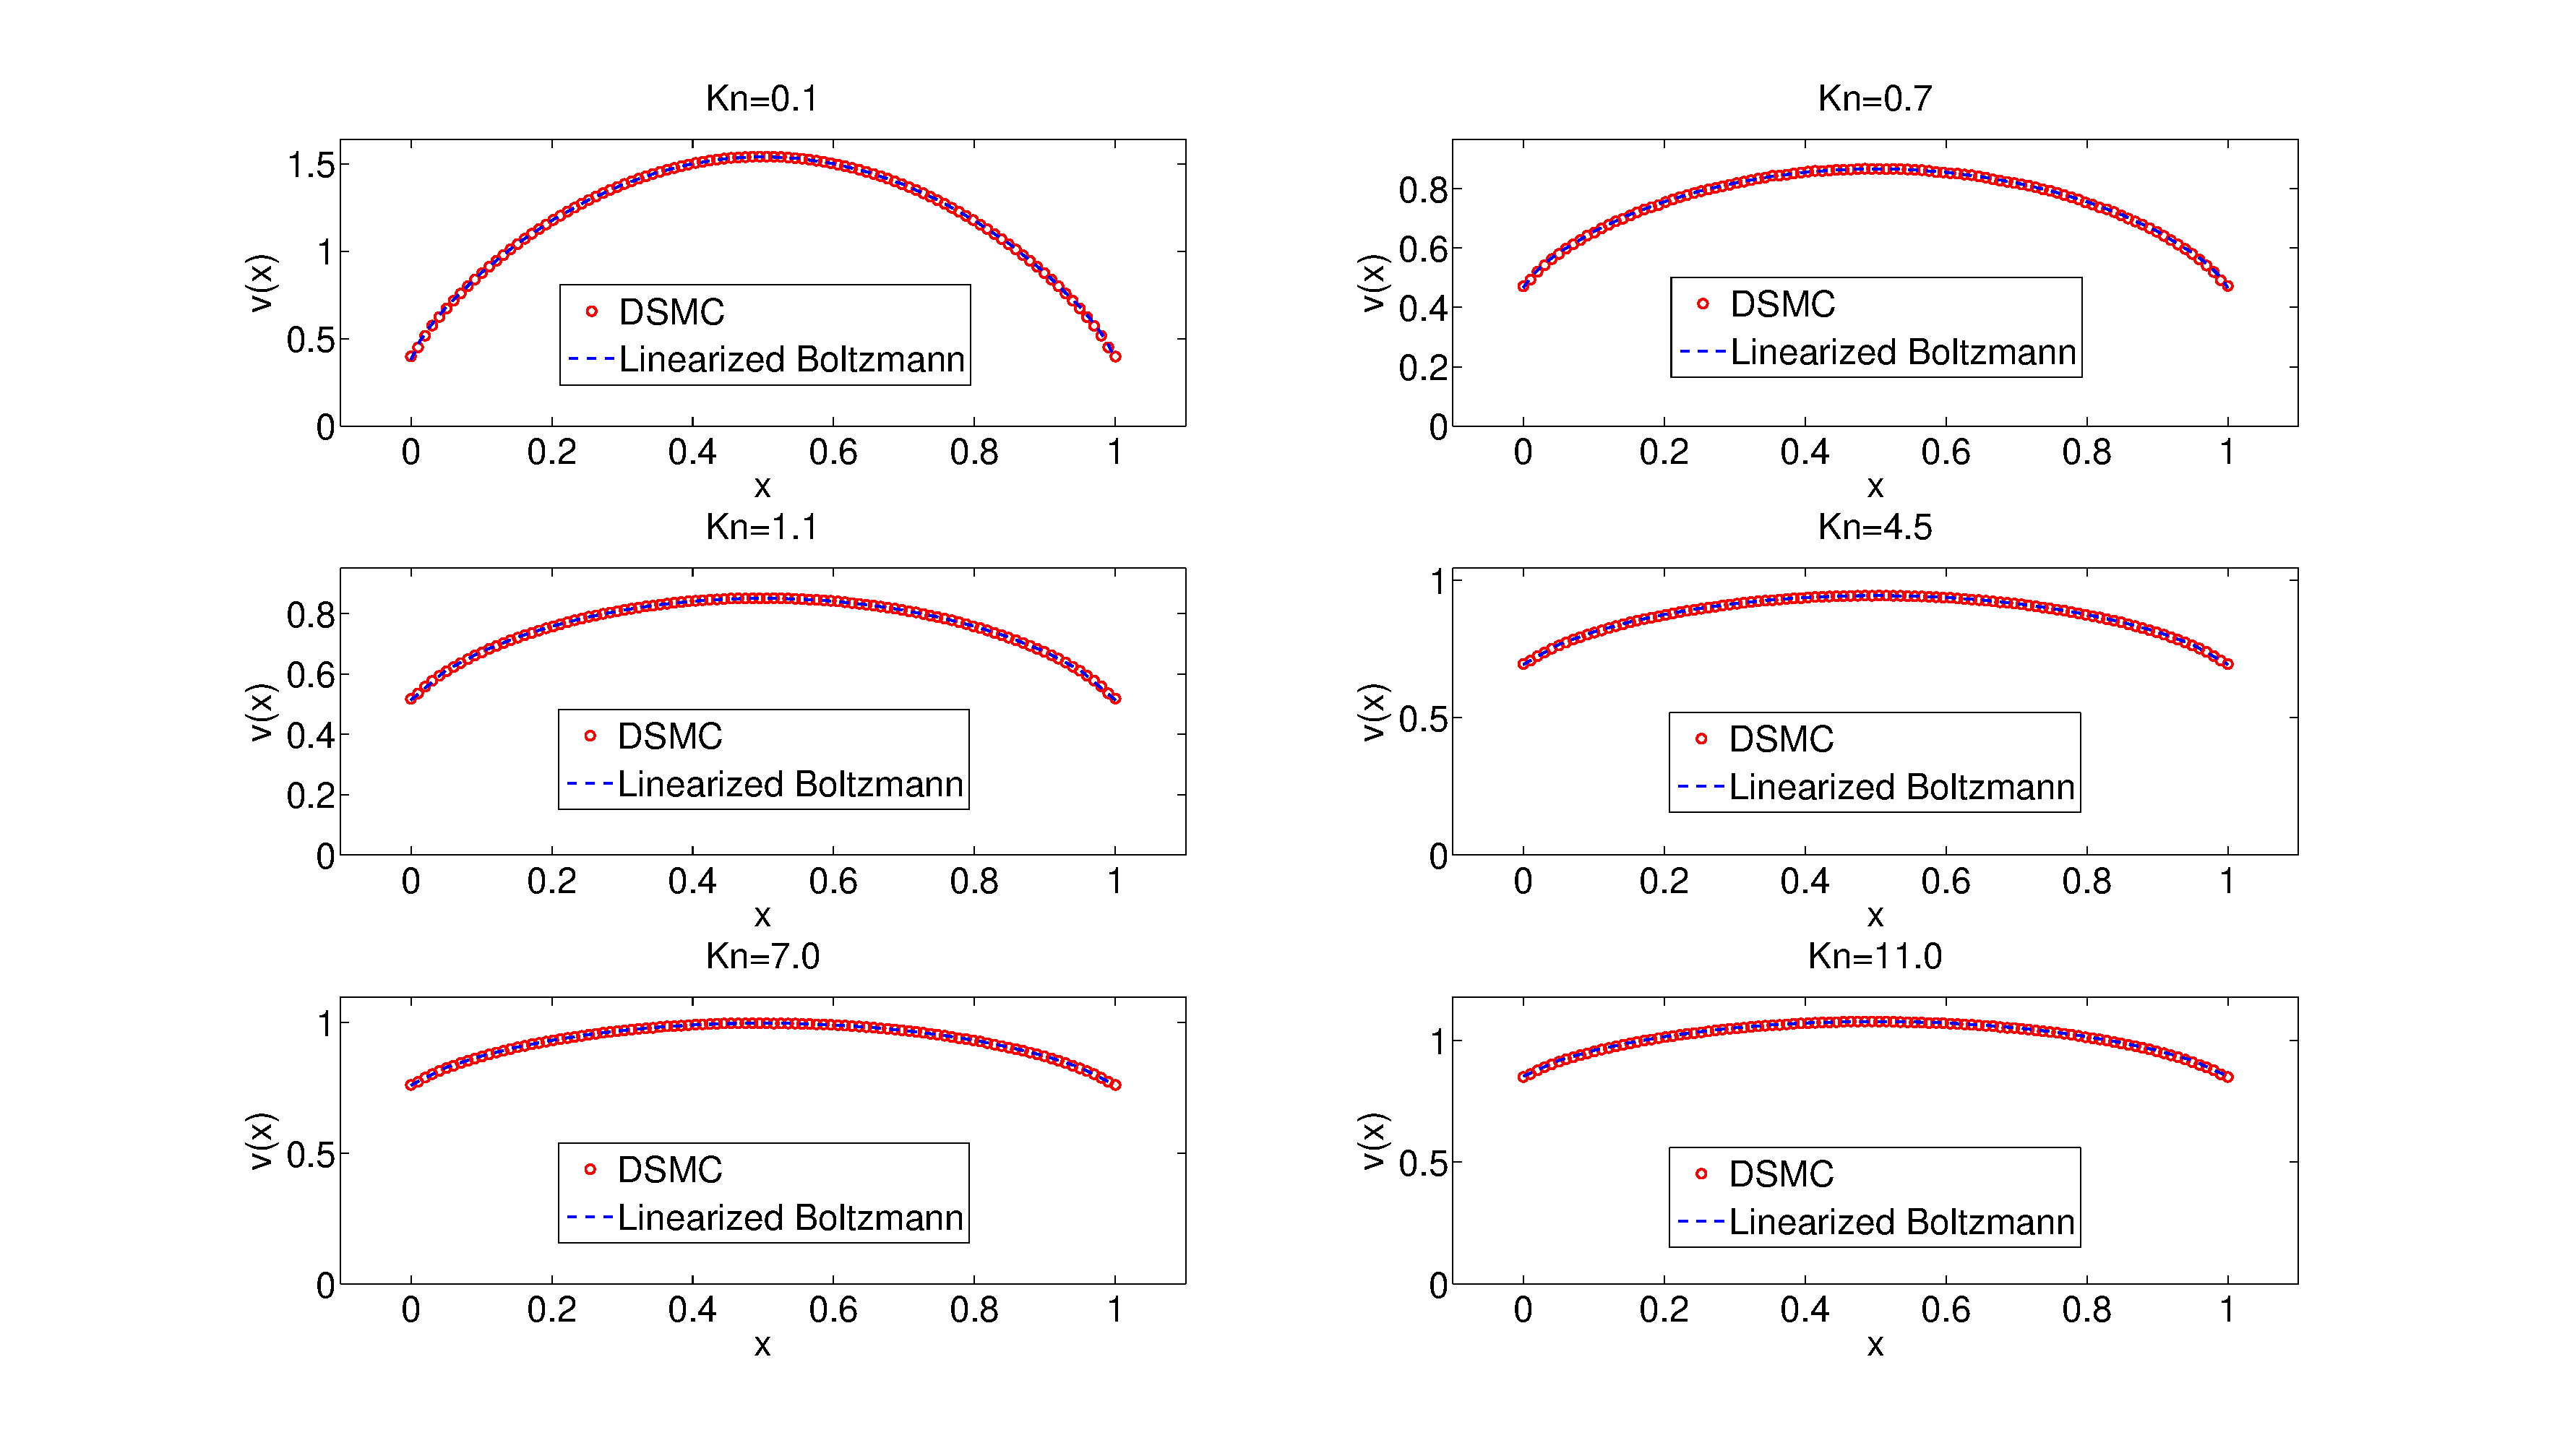
\includegraphics[width=\textwidth, trim=6cm 0cm 5cm 0cm, clip]{DSMC/figures/validation_poiseuille.eps}
\label{fig:dsmc_validation_poiseuille}
\centering
\caption{Nondimensionalized velocity distribution for flow between infinite parallel thermal plates for different Knudsen numbers over two orders of magnitued. Each run is compared to the linearized Boltzmann solution of Ohwada et al\cite{ohwada1989numerical} which shows that the algorithm calculates correctly the behaviour in all regions, near the wall and internally in the channel. $P_A = 1.1P_B, T=300K, V=1\mu m^3$.}
\end{figure}

\subsection{Temperature and pressure profiles}